\section{Method}
\label{method}
In this section we discuss the different methods used in our solution.  We
deconstruct the task of license plate recognition into arbitrary smaller parts.
The first great challenge of license plate recognition is determining the
location of the plate in the picture.  In an upcoming subsection we will
introduce the used bounding box detection system.  The other major challenge of
license plate recognition is actually reading the plate.  After we have assigned
a bounding box the rest is up to an \ac{OCR} subsystem.  An \ac{OCR} recognises
characters printed on the plate.

\subsection{YOLO Object Detection}
We used transfer learning to train a YOLOv7 based on the original implementation
of the paper by \cite{yolov7}. We detect a single object on each image: license
plates. We trained our model for $100$ epochs. We achieved around $90\%$
precision on both training, data and validation data, which carried over to
images of Hungarian license plates as well.

Although the goal of the project is the detect Hungarian license plates, we
observed that a model trained on international license plates generalizes well
enough for the object detection problem. This also made us easier to find
datasets online, as our Hungarian license plate dataset did not include bounding
box data. (See our code repository
\footnote{\url{https://github.com/bobarna/bme-image-processing}} for more
details on the datasets used.)

We used a test data set not seen during training for verifying the model's
generalization capabilities after training. Performance on a randomly sampled
subset of these test images can be seen in Figure~\ref{fig:yolo-test-eval}.

These results show that the model detects the license plates in almost all
cases. Although we can see that the model usually gave a high confidence to the
right detection, while further (usually incorrect) detections have been given
a lower confidence value, we intentionally kept the confidence threshold low in
order not to miss harder to see license plates, even when some other object got
incorrectly recognized with a higher confidence.

\begin{figure}
        \centering
        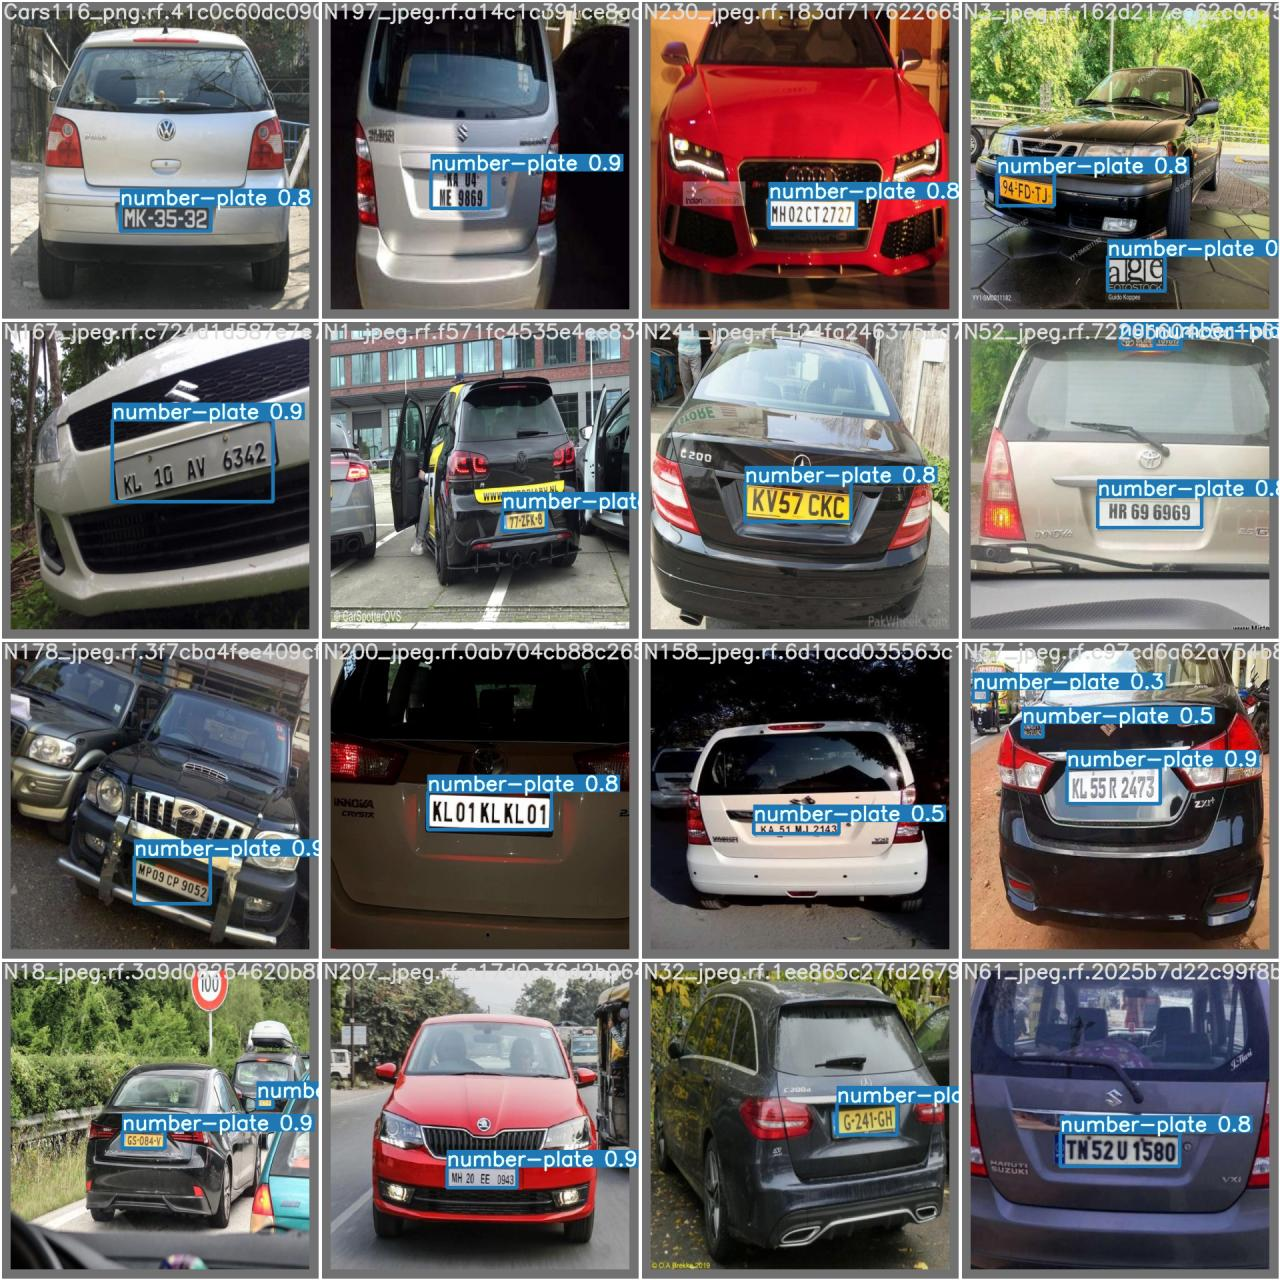
\includegraphics[height=.5\textheight]{figures/transfer-learning-eval/test_batch0_pred.jpg}
        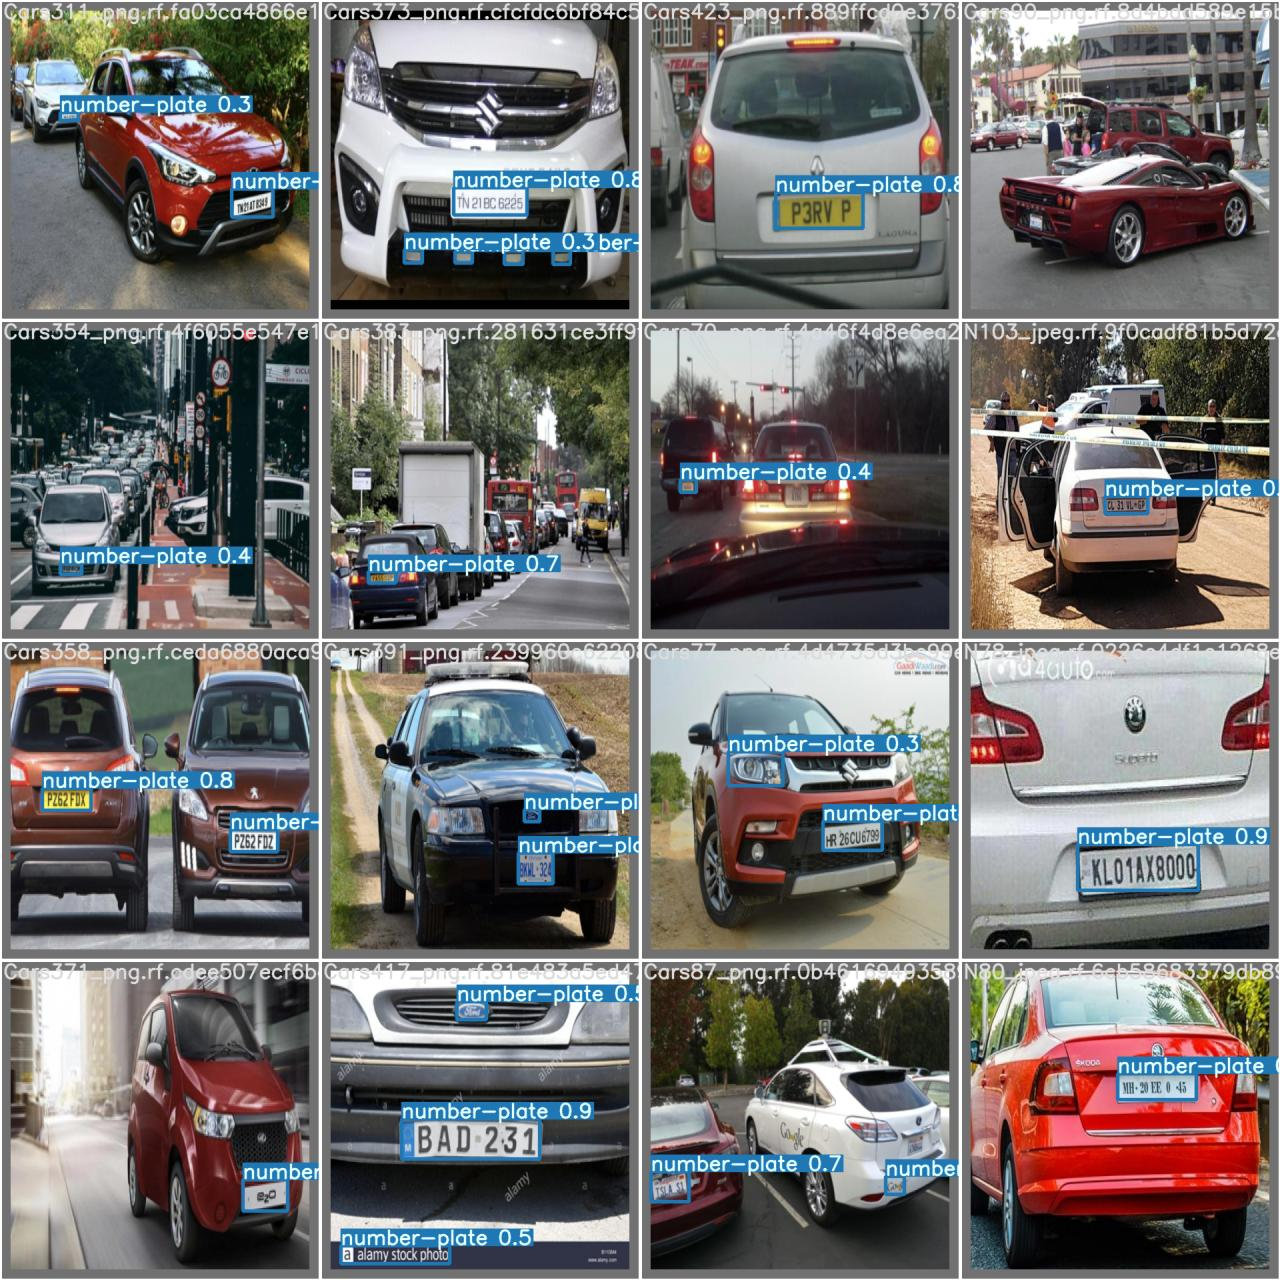
\includegraphics[height=.5\textheight]{figures/transfer-learning-eval/test_batch2_pred.jpg}
        \caption{YOLOv7 transfer learning performance on test data. Confidence
        values are also shown next to each detection.}
        \label{fig:yolo-test-eval}
\end{figure}


\subsection{Data Augmentation via Natural Weather Effects}
We augment our training data for an improved NN learning via natural-looking
weather effects alongside the usual data augmentation strategies.
\begin{itemize}
    \item \emph{light-rain:} A little blur to the image and random generated lines
    \item \emph{normal-rain:} Same as light-rain, but more lines
    \item \emph{snow:} Change the color of some part of picture to white to simulate snow.
    \item \emph{sun:} Increase brigthness for simulating a sunny day
\end{itemize}

We show these effects in action in Figure~\ref{fig:weather-effects}.

\begin{figure}
    \begin{subfigure}[b]{\textwidth}
        \centering
        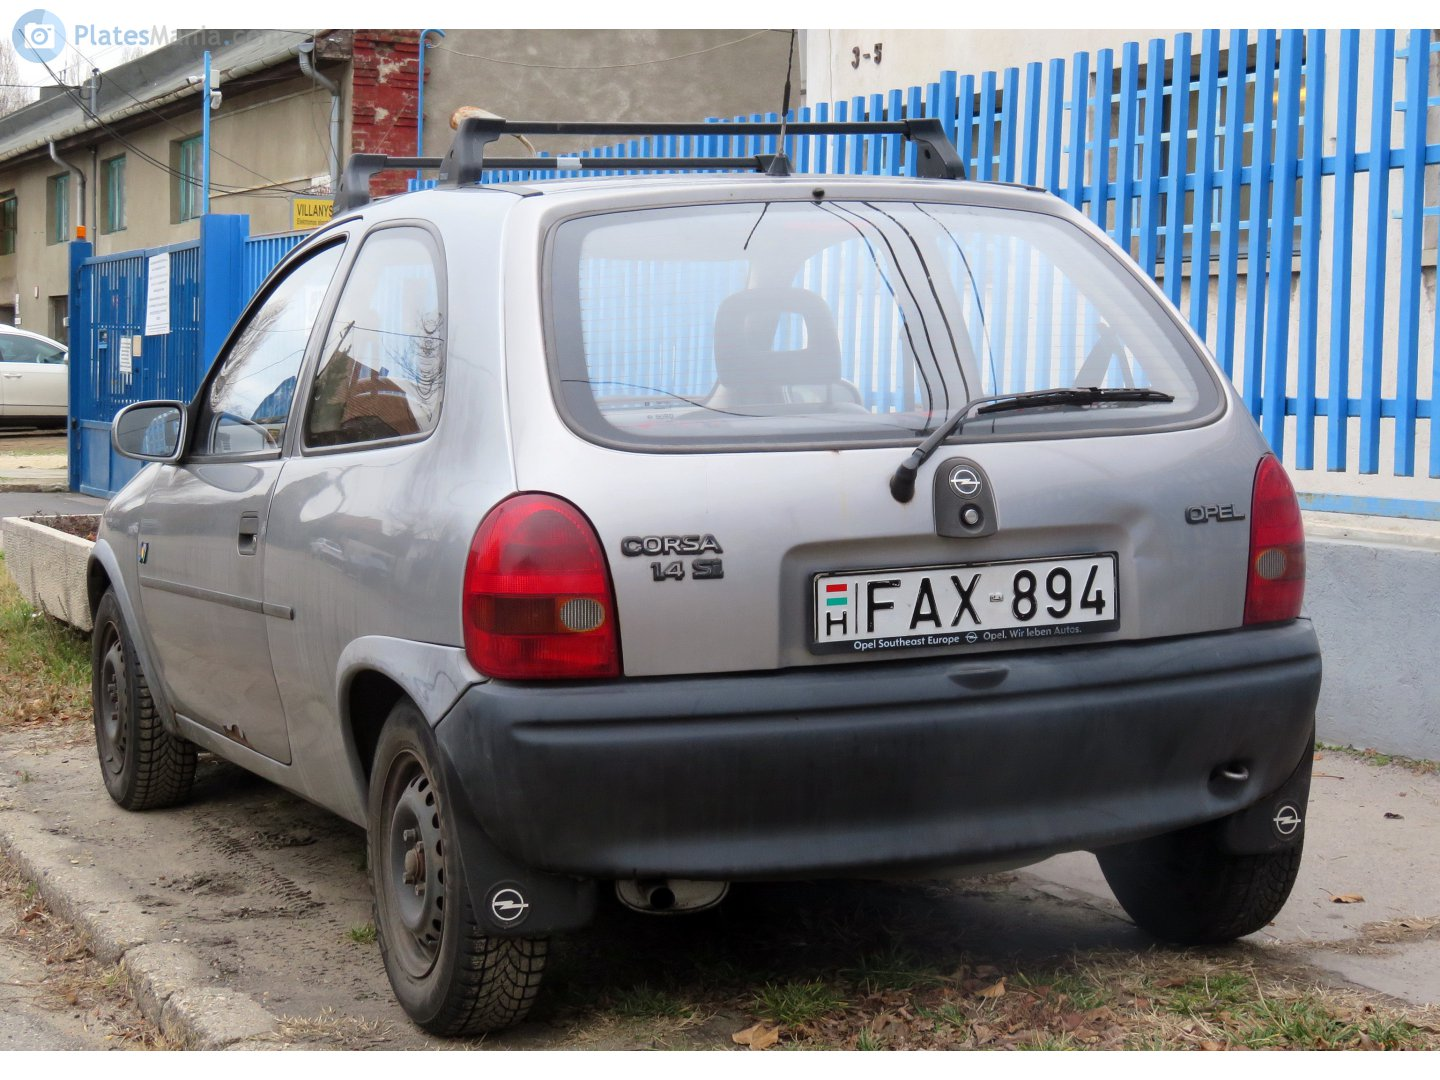
\includegraphics[width=0.45\textwidth]{figures/original.jpg}
        \caption{Original Image}
        \label{fig:weather-original}
    \end{subfigure}
    \begin{subfigure}[b]{\textwidth}
        \begin{subfigure}[b]{.45\textwidth}
            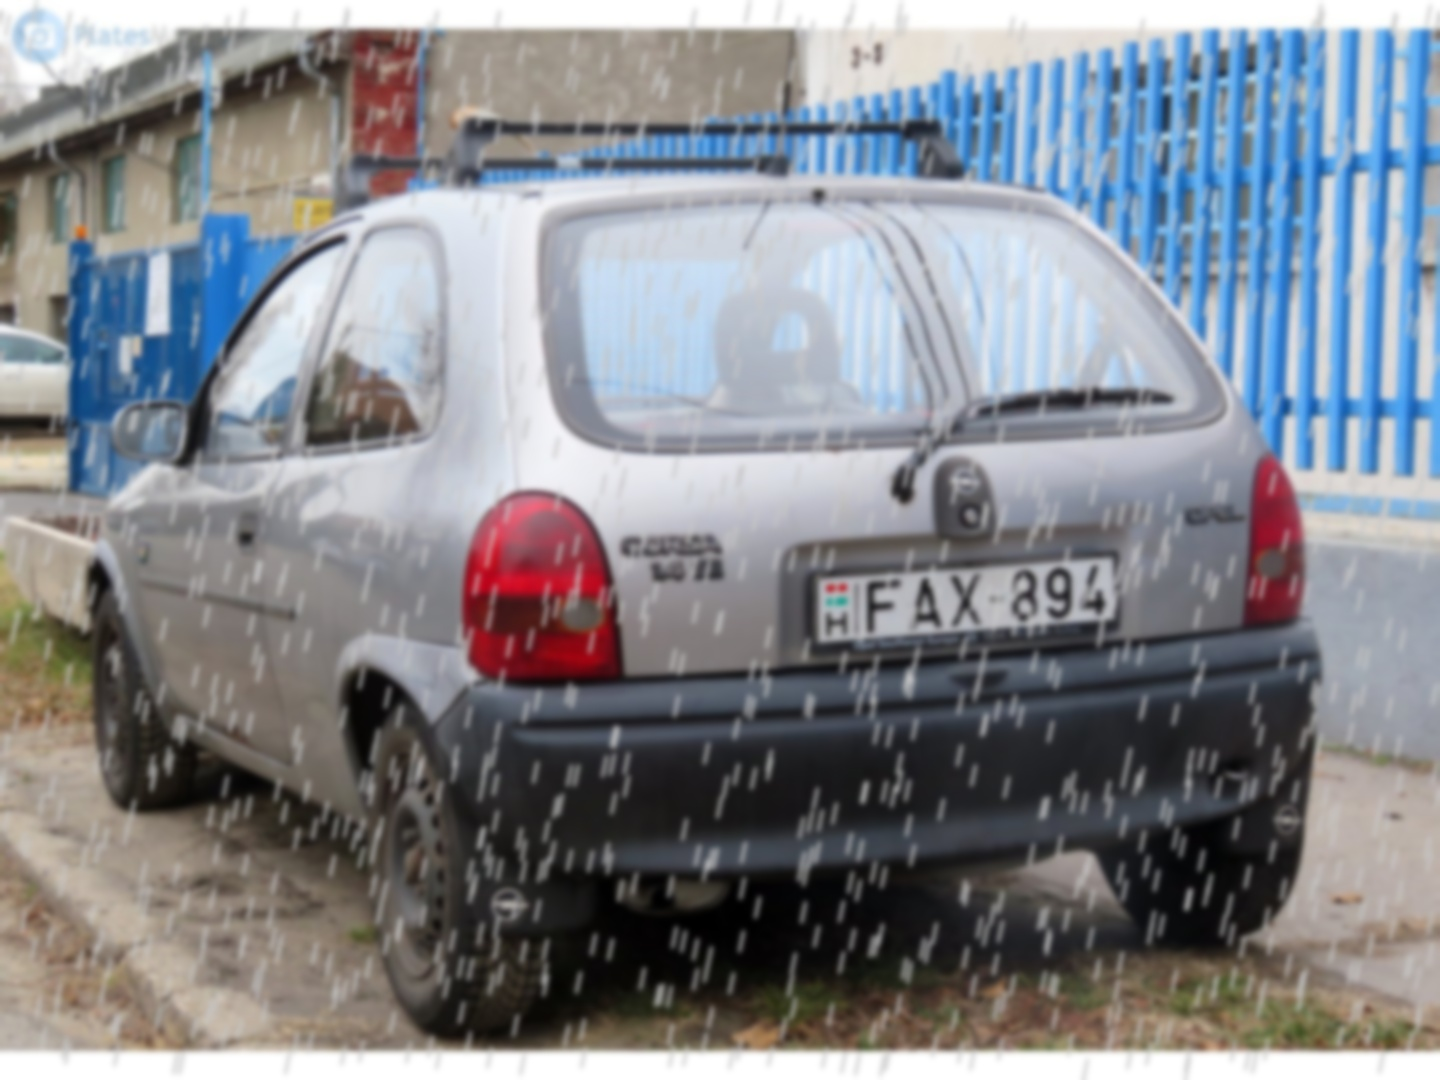
\includegraphics[width=\textwidth]{figures/lightrain.jpg}
        \end{subfigure}
        \hfill
        \begin{subfigure}[b]{.45\textwidth}
            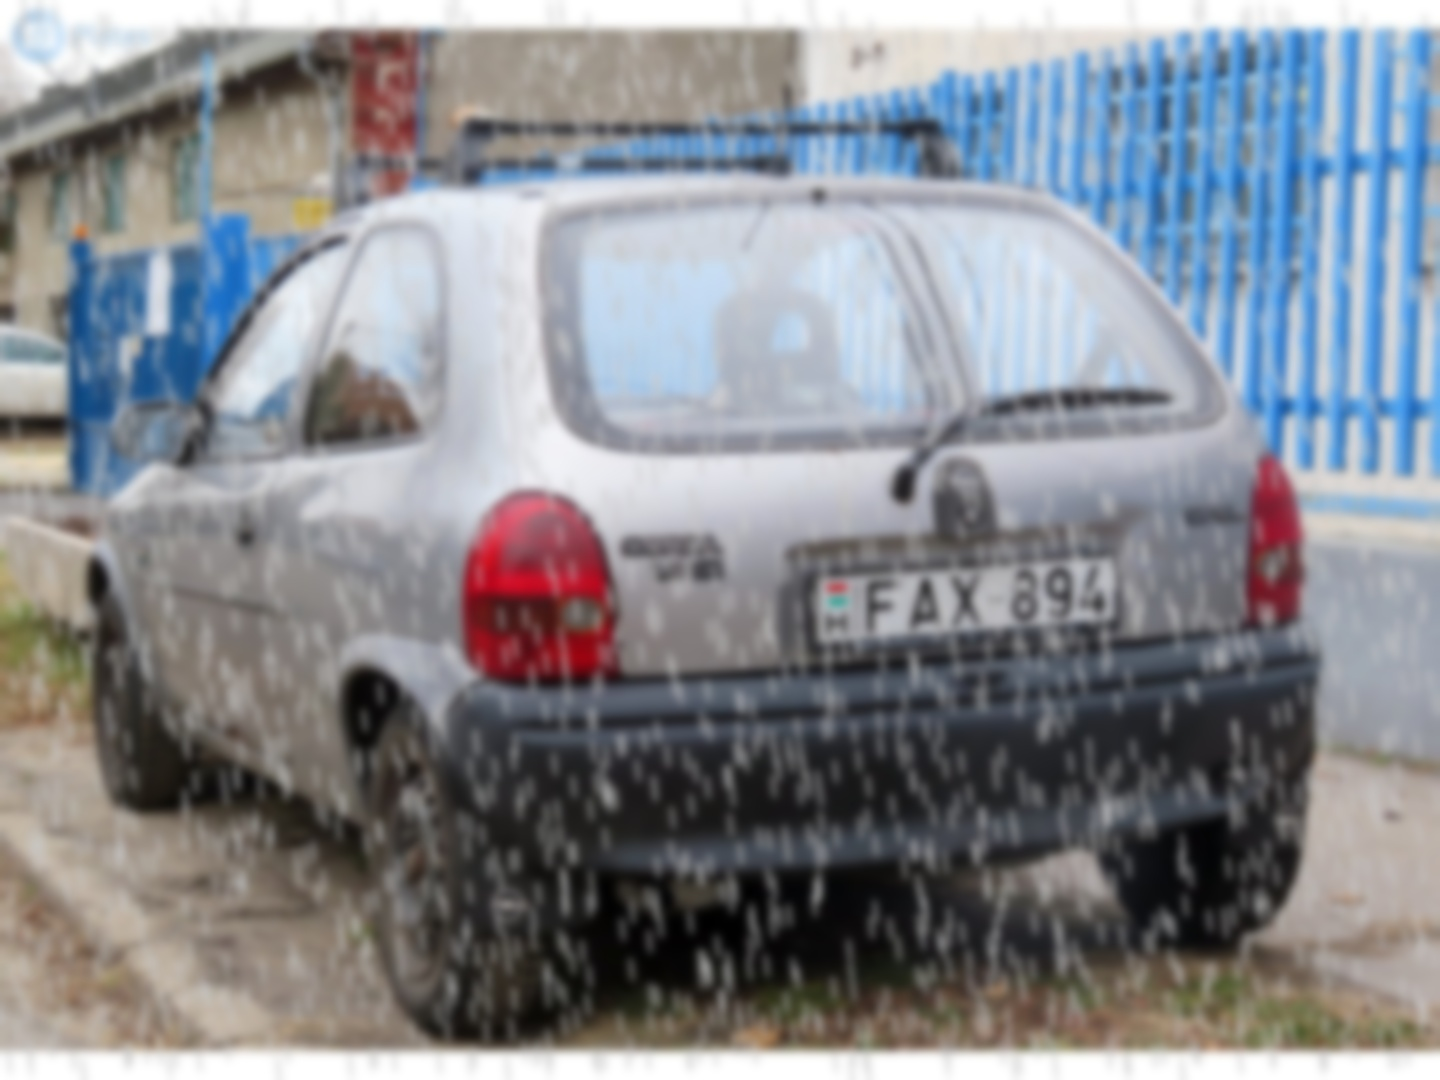
\includegraphics[width=\textwidth]{figures/rain.jpg}
        \end{subfigure}
        \hfill
        \caption{Two types of rain}
        \label{fig:weather-raines}
    \end{subfigure}
    \begin{subfigure}[b]{\textwidth}
        \begin{subfigure}[b]{.45\textwidth}
            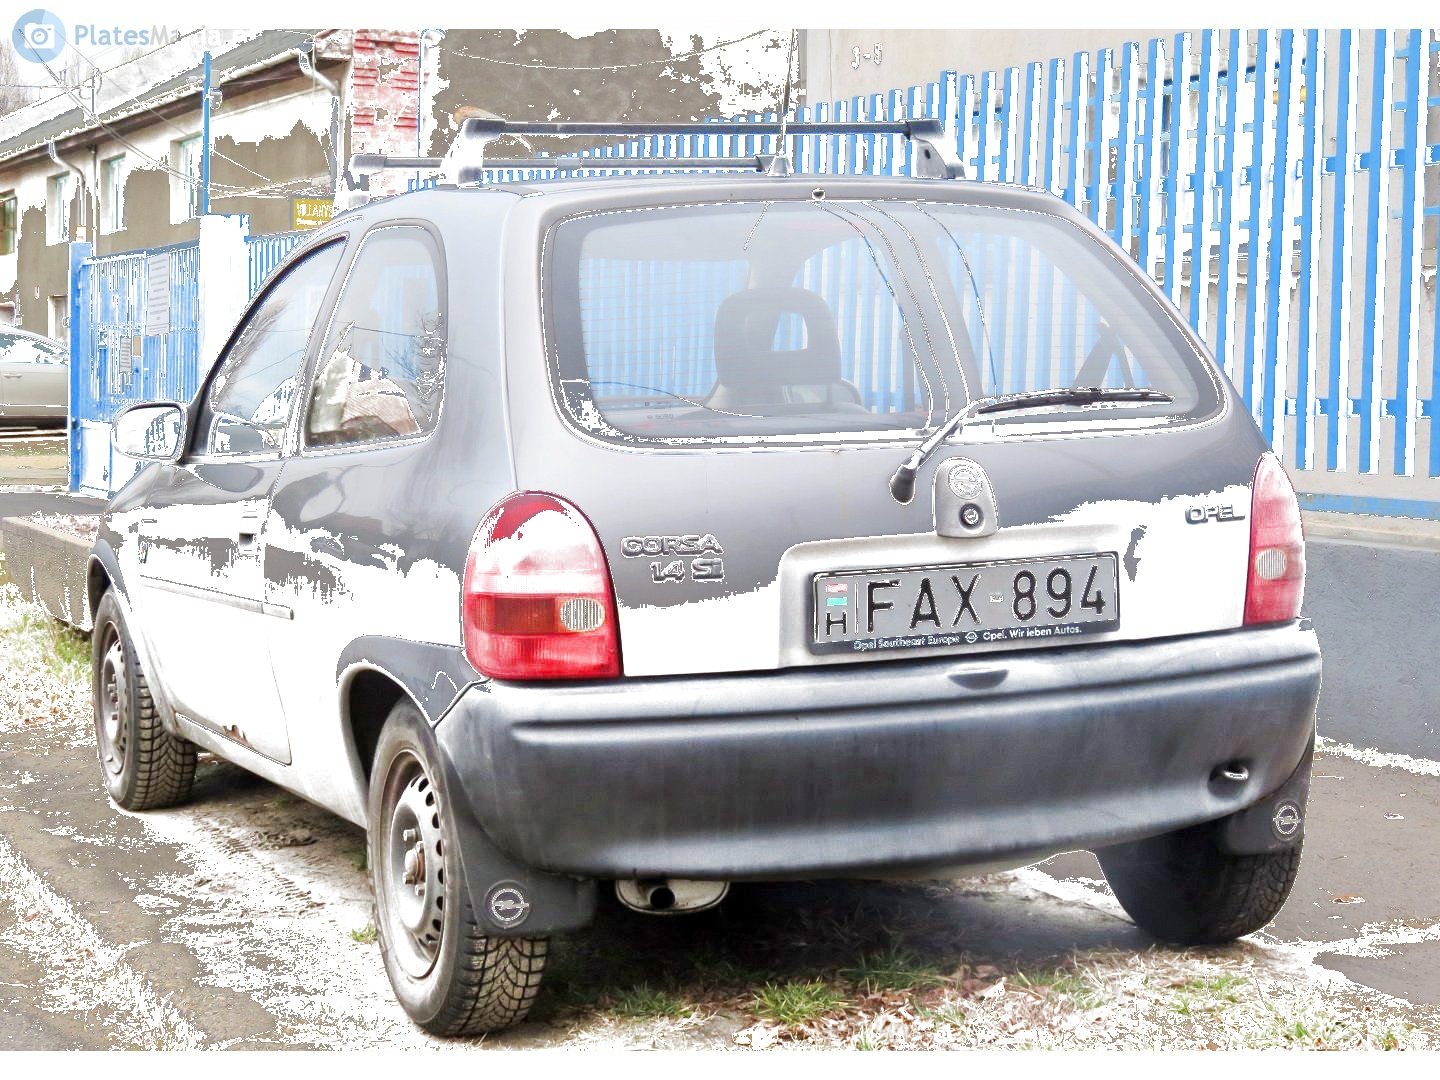
\includegraphics[width=\textwidth]{figures/snow.jpg}
        \end{subfigure}
        \hfill
        \begin{subfigure}[b]{.45\textwidth}
            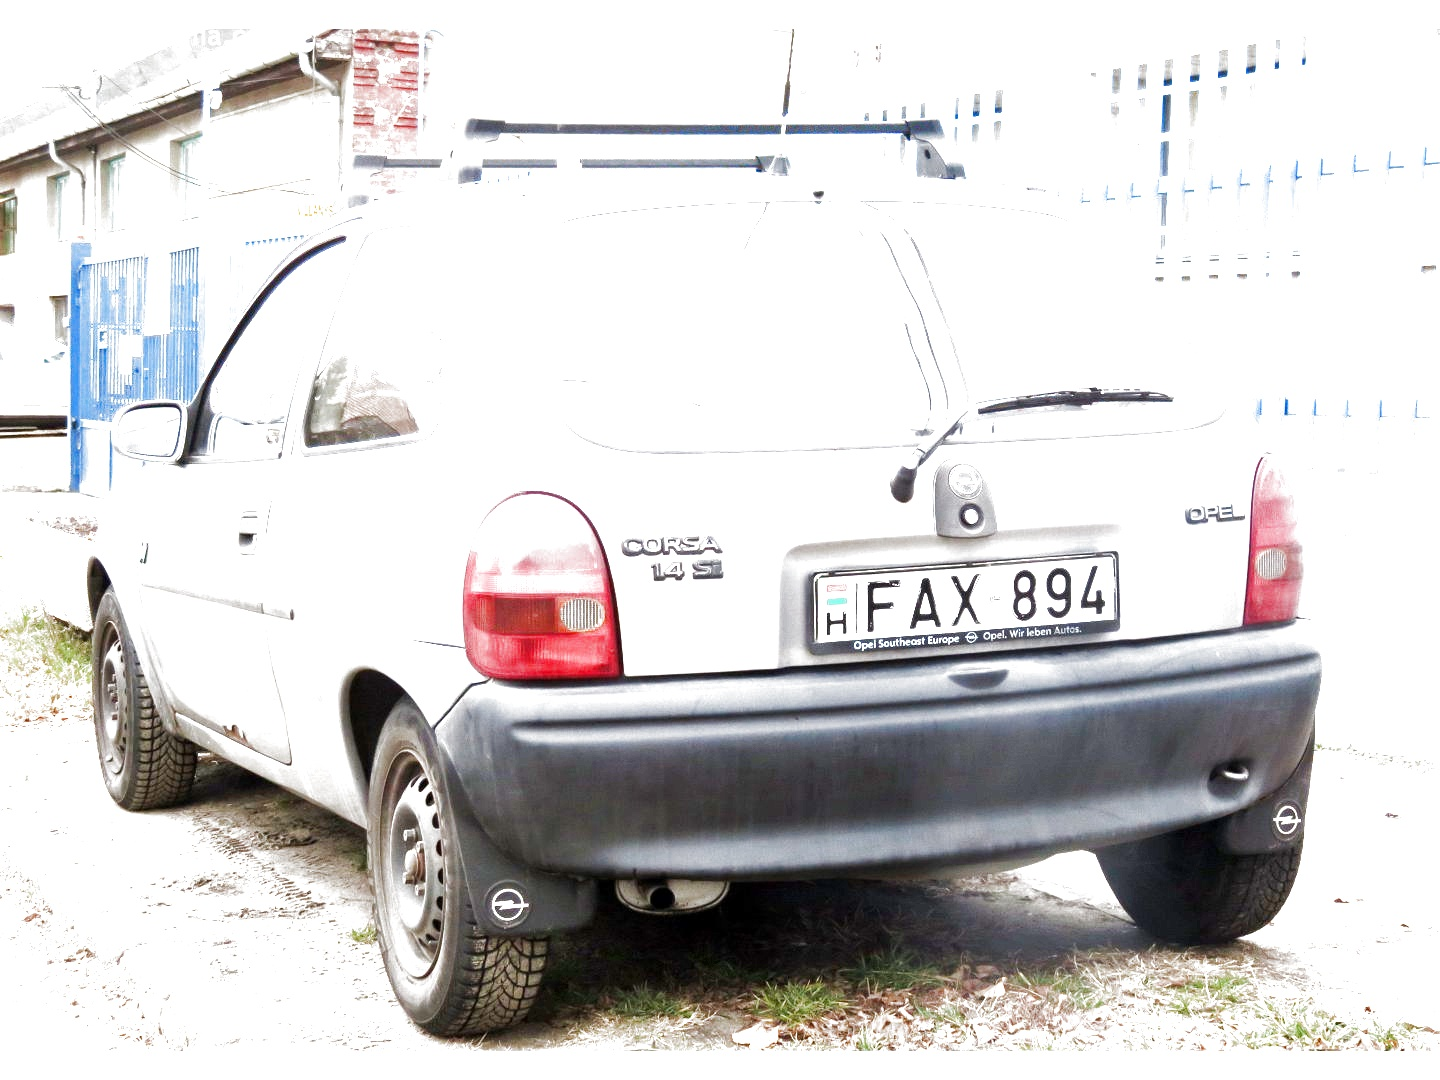
\includegraphics[width=\textwidth]{figures/sunny.jpg}
        \end{subfigure}
        \hfill
        \caption{Snow and Sun filter}
        \label{fig:weather-snow-sun}
    \end{subfigure}
    \caption{Different types of natural-looking weather effects.}
    \label{fig:weather-effects}
\end{figure}

Initially, we implemented these methods following this tutorial: 
\url{https://www.freecodecamp.org/news/image-augmentation-make-it-rain-make-it-snow-how-to-modify-a-photo-with-machine-learning-163c0cb3843f/}.


%--------------------------------------------------
\subsection{Optical~Character~Recognition}
\label{subsec:ocr}
%--------------------------------------------------

In this subsection we discuss the implementation details of the used \ac{OCR} pipeline.
Our work is based on the paper proposed by Shi et al. \cite{7801919}.
\begin{figure}
	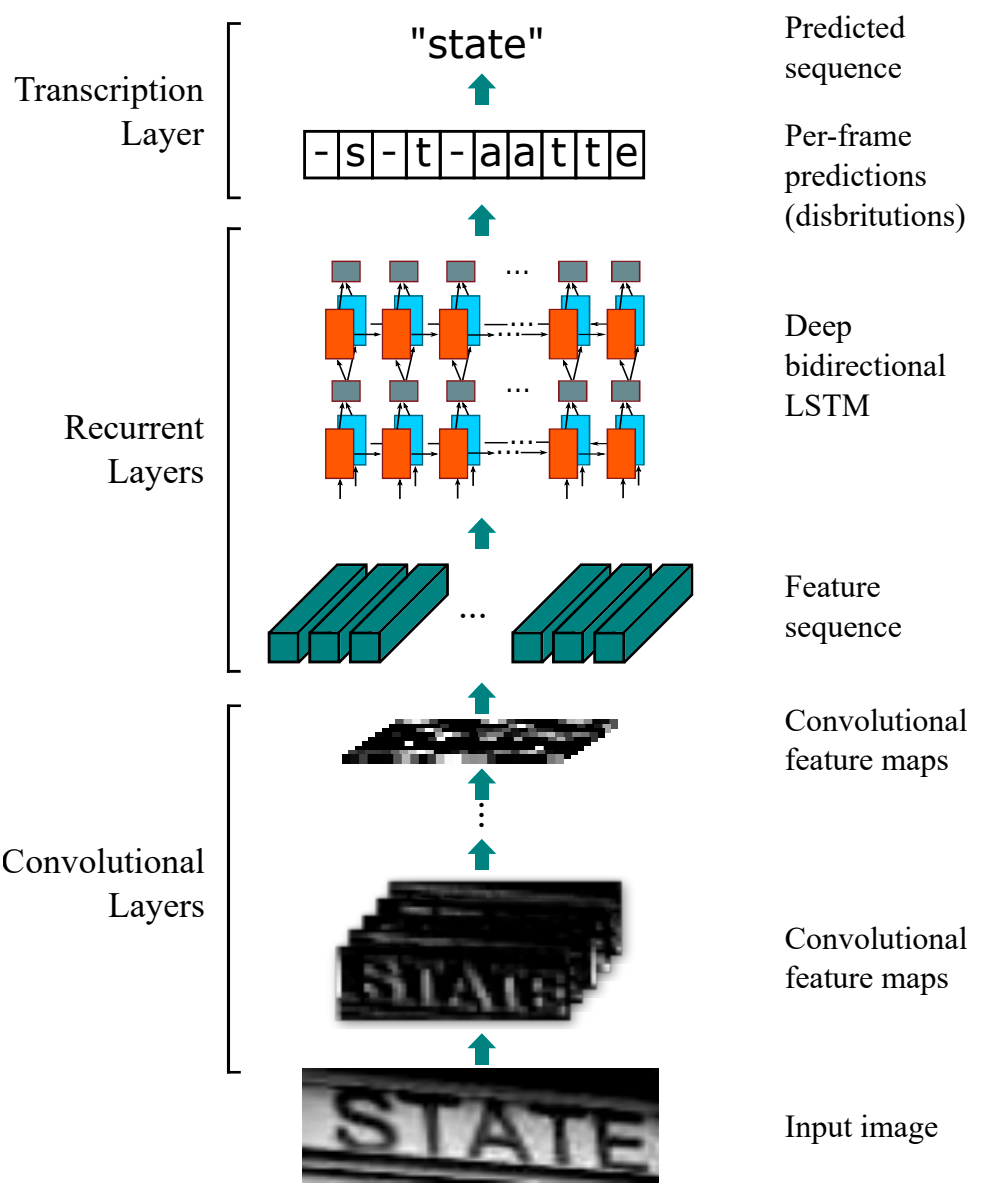
\includegraphics[width=\textwidth]{figures/crnn.png}
	\caption{The architecture published in \cite{7801919}}
	\label{fig:ocr_architecture}
\end{figure}

We deal with the classic problem of computer vision, image-based sequence
recognition. Serial objects, such as scene text, are usually recognized as
a sequence of tags rather than a single tag. RNNs can be trained and optimized
end-to-end, but require complex post-processing steps before being used. CRNN is
a combination of DCNN and RNN and forms an end-to-end system for sequence
recognition. It can be learned directly from sequence labels, does not require
detailed annotations (such as words), and only requires height normalization in
the training and testing sessions.

A CRNN is a type of Recurrent Neural Network (RNN) that can be trained to make
a prediction for each frame of a sequence of features that is output by
convolutional layers. In CRNN, each column of the field maps corresponds to
a region of a rectangle (called the receptive field) of the original image, and
the regions are in the same order as the corresponding columns in the feature
maps from left to right. A deep bidirectional recurrent neural network (CRNN) is
built on top of convolutional layers as recurrent layers.

The recurrent layers predict a label distribution yt for each frame xt of the
feature sequence. Each time it receives a frame in the sequence, it updates its
internal state with a non-linear function that takes both the current input
state and the past state as input. Long-Short-Term Memory (LSTM) is a type of
RNN designed to capture long-range dependencies that often occur in image-based
sequences. LSTM consists of a memory cell and three multiplicative gates, namely
input, output and forget gates. It has made a huge improvement in its speech
recognition function.  Transcription is a process that produces frame-by-frame
predictions into a tag sequence using RNN. Each input in CTC is a sequence
y = y1, ... , yT, where T is the length of the sequence.

We have developed a neural network that can be trained end-to-end on pairs of
images, eliminating the manual labeling of individual components on the training
images. The network is trained with error differences calculated using the
backpropagation algorithm and stochastic gradient descent (SGD).  CRNN is not
limited to recognizing a word in a known dictionary and can handle random
strings ,sentences or other scripts.  The recognition accuracy is plotted as
a function of d. A larger d results in more candidates, thus a more accurate
lexicon-based transcription. On the other hand, the computational cost increases
with larger d, due to the longer BKtree search time. CRNN outperforms commercial
OMR engines such as Capella Scan and PhotoScore by a wide margin.

% here the picture crnn

CRNN uses convolutional features that are highly robust against noise and bias.
It can be easily applied to other image-based sequence recognition
probabilities, requiring minimal domain knowledge.  CRNN, a new neural network
architecture that integrates the advantages of both deep convolutional neural
networks and recurrent neural networks. It runs directly on coarse-level labels
(such as words) and does not require detailed annotations for each eleventh
(i.e., character) in the training phase.








\subsection{Preprocessing for OCR}

After cutting the license plate we apply some preprocessing method with OpenCV:
\begin{itemize}
    \item \emph{Normalization:} using the \texttt{cv2.normalize} method.
    \item \emph{Noise removal:} using the
        \texttt{fastNlMeansDenoisingColored} function of OpenCV.
    \item \emph{Erodation:} using a $5 \times 5$ kernel matrix of ones.
    \item \emph{Blur clarification:} for the blur clarification, we used a matrix
        with a value $9$ center surrounded with $-1$ values.
    \item \emph{Adaptive Threshold:} using the \texttt{adaptiveThreshold}
        function of OpenCV. 
\end{itemize}

This results in a much better image for the OCR, converting the image to
grayscale and sharpening the label of the license plate. 

\begin{align*}
    \text{Kernel}_{\text{erodation}}&= 
    \begin{bmatrix}
        1 & 1 & 1\\
        1 & 1 & 1 \\
        1 & 1 & 1
    \end{bmatrix}\\
    \text{Kernel}_{\text{blur clarification}}&= 
    \begin{bmatrix}
        -1 & -1 & -1\\
        -1 & 9  & -1 \\
        -1 & -1 & -1
    \end{bmatrix}
\end{align*}

\begin{figure}
    \begin{subfigure}[b]{.45\textwidth}
        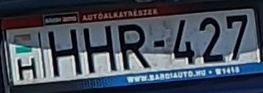
\includegraphics[width=\textwidth]{figures/preprocessbefore1.jpg}
    \end{subfigure}
    \hfill
    \begin{subfigure}[b]{.45\textwidth}
        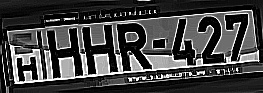
\includegraphics[width=\textwidth]{figures/preprocessafter1.jpg}
    \end{subfigure}
    \hfill
    \\
    \begin{subfigure}[b]{.45\textwidth}
        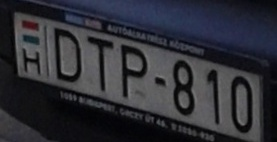
\includegraphics[width=\textwidth]{figures/preprocessbefore2.jpg}
    \end{subfigure}
    \hfill
    \begin{subfigure}[b]{.45\textwidth}
        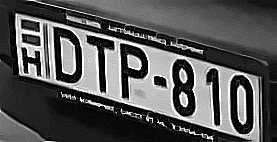
\includegraphics[width=\textwidth]{figures/preprocessafter2.jpg}
    \end{subfigure}
    \hfill
    \\
    \begin{subfigure}[b]{.45\textwidth}
        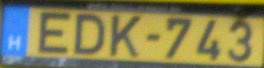
\includegraphics[width=\textwidth]{figures/preprocessbefore3.jpg}
    \end{subfigure}
    \hfill
    \begin{subfigure}[b]{.45\textwidth}
        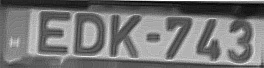
\includegraphics[width=\textwidth]{figures/preprocessafter3.jpg}
    \end{subfigure}
    \hfill
    \caption{Preprocessing results.}
    \label{fig:preprocessing-fig}
\end{figure}

